
\noindent\textbf{4. (CRLS 22.2-5)} Considere um grafo orientado $D = (N, A)$. Dê um exemplo de um conjunto $A_\pi \subseteq A$ de arcos em $D$ que formam uma árvore tal que, entre quaisquer dois nós $u$ e $v$ em $D$, o único caminho entre $u$ e $v$ em $A_\pi$ é um caminho mínimo em $D$ entre $u$ e $v$, porém, $A_\pi$ jamais seria produzida por uma execução da BFS em $D$, independente da ordem dos nós nas listas de adjacências de $D$ e do nó inicial $s$.

\textbf{Resposta:} Seja o conjunto de arcos $A_\pi$ destacados no grafo da figura \ref{fig:7.4-1}.
\begin{center}

\includegraphics[width=0.8\textwidth]{q7-04-p1.png}
\captionof{figure}{Grafo orientado $D = (N, A)$.}
\label{fig:7.4-1}
\end{center}

Note que, independente da ordem dos elementos adjacentes a $s$, $t$ e $u$, essa representação jamais poderá ser obtida pela \proc{BFS}. A ordem das listas de adjacências dos elementos $t$ e $u$ também não influenciam na forma com que a árvore será gerada. A figura \ref{fig:7.4-2} mostra o resultado da execução da \proc{BFS}, bem como a lista de adjacências em ordens diferentes em cada caso.
\begin{center}
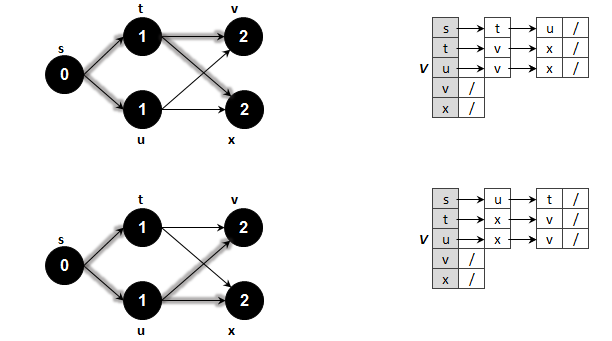
\includegraphics[width=0.8\textwidth]{q7-04-p2.png}
\captionof{figure}{Execução da \proc{BFS} no grafo orientado $D = (N, A)$ com a lista de adjacências em duas ordens distintas.}
\label{fig:7.4-2}
\end{center}
